El objetivo de esta sección es presentar un escenario sencillo para mostrar cómo el uso de EPAs puede ayudar a un auditor a ganar conocimiento sobre contratos inteligentes que no escribió, y de los que no cuenta ninguna especificación formal.
El ejemplo es extraído del artículo publicado por Godoy et al. en 2022\cite{predicate-abstraction-for-smart-contract-validation}, y se refiere a una implementación de \texttt{Crowdfunding} perteneciente a la librería de contratos de OpenZeppelin durante 2022 \cite{open-zeppelin-library}.
Las figuras utilizadas son provenientes del trabajo publicado por Torres et. al en 2023\cite{Torres}.

Supongamos que un auditor ofrece servicios de auditoría de contratos inteligentes como contratista, y accede a evaluar un contrato de un cliente.
El cliente quiere desplegar un contrato en una blockchain que se encargue de recaudar el dinero que necesitará para su próximo proyecto.
Cuenta con una implementación de este contrato, pero la comunidad de inversores exige que el contrato sea validado por un experto para corroborar que hace lo prometido con el dinero.
Por este motivo, el cliente provee el código fuente al auditor y una descripción burda del comportamiento deseado:
\begin{itemize}
    \item Al desplegar el contrato, se debe anunciar el objetivo deseado (en dinero a recaudar) y la fecha límite hasta la que estará abierta la recaudación.
    \item La comunidad de inversores puede contribuir hacia la meta con cuanto dinero desee, siempre y cuando no se haya alcanzado la fecha límite.
    \item De alcanzarse la meta a tiempo, entonces el cliente podrá recolectar todo el dinero recaudado.
    \item Si la recaudación llega a su fecha límite sin haber alcanzado la meta, entonces el cliente pretende garantizar a los inversores que podrán recuperar todo su dinero.
    \item Sin embargo, antes de la fecha límite ni los inversores ni el cliente pueden retirar dinero, para garantizar transparencia de cuál es el porcentaje de avance hacia la meta.
\end{itemize}

El auditor comienza su trabajo sobre la implementación del contrato \texttt{Crowdfunding} (cuyo código podemos ver en el fragmento \ref{code:crowdfunding-solidity}).
Puede observar que aparte del constructor inicial, está programado con tres métodos: \texttt{Donate}, \texttt{GetFunds} y \texttt{Claim}.
Debido a que estos no son muy complejos puede rápidamente ver que están bien nombrados; cada uno se corresponde con una de las acciones descritas por el cliente que se desea que se puedan hacer en la recaudación.
Sin embargo, es crucial corroborar que estos métodos estén habilitados de la manera que el cliente desea.
Para realizar este análisis el auditor utiliza una herramienta automática que abstrae el contrato a una máquina de estados finita, que podemos ver en la figura \ref{fig:crowdfunding-epa}

\begin{figure}
    \centering
    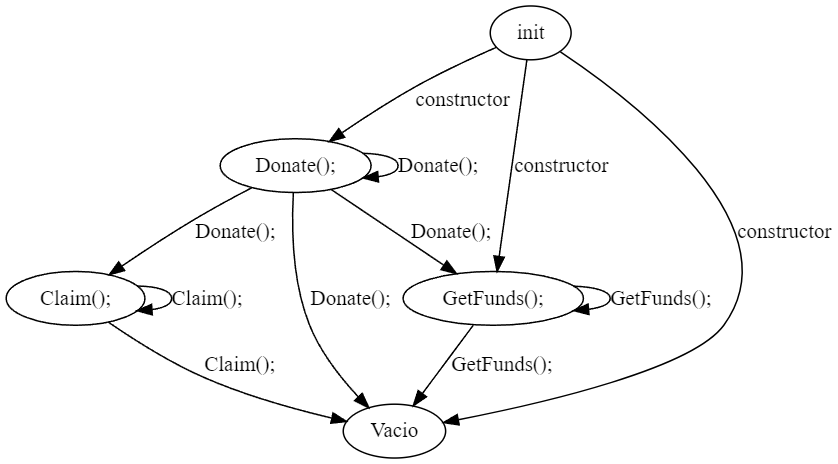
\includegraphics[width=0.75\textwidth]{figs/crowdfunding-epa.png}
    \caption{Enabledness Preserving Abstraction del contrato \texttt{Crowdfunding} }
    \label{fig:crowdfunding-epa}
\end{figure}

Esta máquina de estados se corresponde razonablemente bien con las etapas en la recaudación que describe el cliente.
Por ejemplo, podemos ver que desde el estado en el que se puede donar (el etiquetado como \texttt{Donate}) es posible donar múltiples veces.
Además, es posible donar y transicionar a un estado en el que lo unico que se puede hacer es que el cliente reclame los fondos (el etiquetado como \texttt{Claim}) o a un estado donde lo unico que se puede hacer es que los inversores recuperen su dinero (el etiquetado como \texttt{GetFunds}).

De esta manera, el auditor puede observar todos los caminos que son posibles en la abstracción y contrastarlos con los caminos que piensa que deberían ser posibles dada la descripción del cliente.
Aún más, al analizar la abstracción puede buscar caminos que le resulten sospechosos; que parezcan indicar que es posible una secuencia de ejecuciones que no resulta deseable en base a la especificación con la que cuenta.
Por ejemplo, al auditor podrían llamarle la atención las transiciones que llevan al estado etiquetado como ``\texttt{Vacío}'', ya que no desea que el contrato pueda bloquearse.
Sospechando que la causa de este estado ``\texttt{Vacío}'' en realidad son detalles en la implementación con respecto al manejo del tiempo (recordemos que el auditor es un experto), le pide a la herramienta que genere una nueva abstracción en que modele el paso del tiempo, como la que podemos ver en la figura \ref{fig:crowdfunding-time-epa}

\begin{figure}[h]
    \centering
    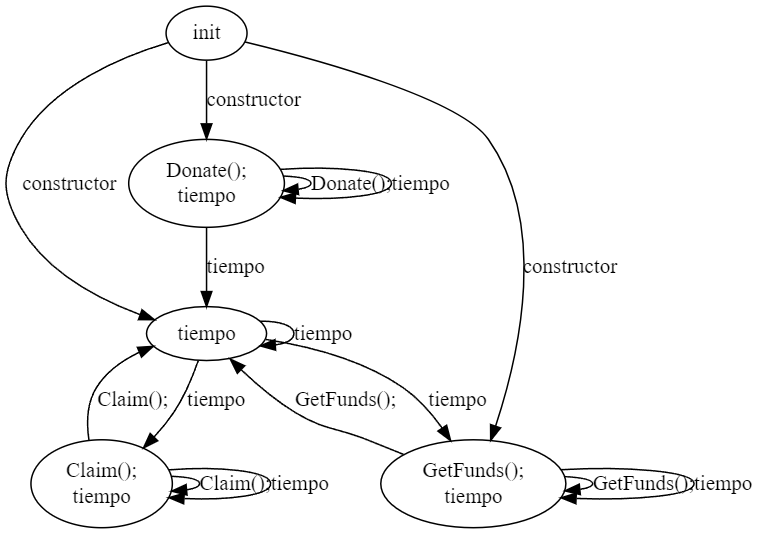
\includegraphics[width=0.75\textwidth]{figs/crowdfunding-time-epa.png}
    \caption{Abstracción del contrato \texttt{Crowdfunding} basada en la EPA, que además modela el paso del tiempo.}
    \label{fig:crowdfunding-time-epa}
\end{figure}

Al observar esta nueva máquina de estados, el auditor puede confirmar su sospecha de que el estado ``\texttt{Vacío}'' en realidad era un estado al que se puede entrar y salir con el paso del tiempo.
Sin embargo su trabajo no está terminado; debe poner a prueba todos los escenarios que se le ocurran hasta garantizar que el dinero de todos los participantes esté a salvo.
Por ejemplo, podría continuar refinando la abstracción pidiéndole a la herramienta que divida los estados del contrato en base a si el contrato controla dinero o no, ya que el único caso problemático sería que el contrato se bloquee cuando controla dinero de las otras personas.

A grandes rasgos, podemos decir que este procedimiento de generar abstracciones y refinarlas permite al auditor validar el comportamiento del contrato.
Hace esto enfocándose en casos de uso o ejecución complejos, pero puede hacerlo sin depender de análisis manuales intensivos del código fuente, que son propensos a errores.

\begin{lstlisting}[language=Solidity, label={code:crowdfunding-solidity}, caption=Implementación de la recaudación]
contract Crowdfunding {
    address payable owner;
    uint max_block;
    uint goal;
    mapping (address=>uint) backers;
    bool funded = false;
    
    constructor (address payable _owner, uint _max_block, int _goal) public {
        owner = _owner;
        max_block = _max_block;
        goal = _goal;
    }
    function Donate () public payable {
        require (max_block > block.number);
        require (backers [msg.sender] == 0);
        backers [msg.sender] = msg.value;
    }
    function GetFunds () public {
        require (max_block < block.number);
        require (msg.sender == owner);
        require (goal <= address(this).balance);
        funded = true;
        owner.transfer(address(this).balance);
    }
    function Claim () public {
        require (max_block < block.number);
        require (backers [msg.sender] > 0 && ! funded);
        require (goal > address (this).balance);
        uint val = backers [msg.sender];
        backers [msg.sender] = 0;
        msg.sender.transfer (val);
    }
}
    
\end{lstlisting}